%!TEX root = ../main.tex

% \part{Enhancing the System Stability Assessment}

%%%%%%%%%%%%%%%%%%%%%%%%%%%%%%%
%%%%%%%%%%%%%%%%%%%%%%%%%%%%%%%
\chapter{Verification Setup and Results}
\label{chap:verification}

\begin{textblock*}{.7\textwidth}(70mm-\offset,25mm-\offset)
    \begin{fquote}[Mark Twain]
        If you tell the truth, you don't have to remember anything.
    \end{fquote}
\end{textblock*}

%%%%%%%%%%%%%%%%%%%%%%%%%%%%%%%
\section{Representative Electrical Networks}

The following section shall introduce the used power systems in the simulation with the Python framework, considering verification, and also extension meaning the performed case studies in \autoref{chap:case-study}. The models are chosen to represent different network sizes and complexities, thus allowing the objective of graded interaction levels of the developed (transformer) model. The models are based on the work of \textcite{machowskiPowerSystemDynamics2020}, \textcite{kundurPowerSystemStability2022}, \textcite{IEEEGuideLoad2022}, and \textcite{vancutsemTestSystemsVoltage2020}.

\subsubsection{Single Machine Infinite Bus (SMIB) Model}

One very popular and thus powerful electrical network for the verification of power system stability is the \acs{SMIB} model. It is a compact and simplified model of a power system, allowing easy analytical calculation, verification and development. Mutual influences are comparably simple to understand and calculate, as the infinite bus bus is acting as a fixed grid connection point with a large adjoining grid. The generator is connected to the bus bar via a transmission line and a transformer. The model was largely discussed by \textcite{kundurPowerSystemStability2022}, and is shown in Figure \ref{fig:smib-model}. The generator and the \acs{IBB} are represented by synchronous machines, developed and discussed by \textcite{kordowichPhysicsInformedMachine2023}. The specific model details are included in \autoref{app:smib-model}, additionally the simulation setup for verification is described in \autoref{tab:smib-model}.

\begin{figure}[htb]
    \centering
    \vspace{12pt}
    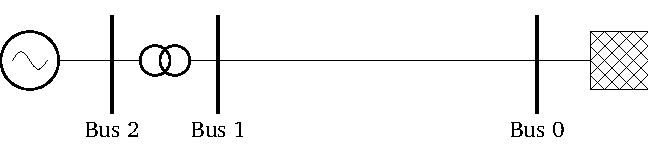
\includegraphics{tikz_graphics/images/smib_model.pdf}
    \vspace{12pt}
    \caption[]{\acf{SMIB} model for verification and validation of the Python framework; own figure after \autocite{machowskiPowerSystemDynamics2020,kundurPowerSystemStability2022}}
    \label{fig:smib-model}
\end{figure}

\begin{table}[htb]
    \caption[Simulation Setup for validation of the $\Pi$-modeled transformer]{Simulation Setup for validation of the $\Pi$-modeled transformer; considering a transforming ratio $\underline{\vartheta} \neq 1$ and $\underline{\vartheta} \in \mathbb{C}$}
    \label{tab:smib-model}
    \vspace*{12pt}
    \centering
    \small
    \begin{tabularx}{\textwidth}{Xr}
        % \toprule
        \textbf{Parameter} & \textbf{Value} \\ \hline
        \toprule
        Generator inertia $H$ & 3.5 s \\
        Generator damping $D$ & 0.1 p.u. \\
        Generator resistance $R$ & 0.01 p.u. \\
        Generator reactance $X$ & 0.1 p.u. \\
        Transformer resistance $R$ & 0.01 p.u. \\
        Transformer reactance $X$ & 0.1 p.u. \\
        Transmission line resistance $R$ & 0.01 p.u. \\
        Transmission line reactance $X$ & 0.1 p.u. \\
        \bottomrule
    \end{tabularx}
\end{table}

Further, this model shall be slightly modified according to \autoref{fig:smib-model-mod}. A load is added at the secondary bus of the transformer, the rest of the system is kept. \autoref{tab:smib-model} already contains this modification.

\begin{figure}[htb!]
    \centering
    \vspace{12pt}
    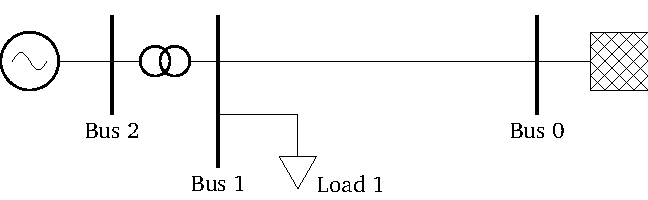
\includegraphics{tikz_graphics/images/smib_model_with_load.pdf}
    \vspace{12pt}
    \caption[]{Modified \acf{SMIB} model with additional load}
    \label{fig:smib-model-mod}
\end{figure}

\subsubsection{Simple Single Machine Load Model}

Following model is often recommended \quelle for easy voltage control studies, in explicit for \acsp{OLTC}. Similar to the \acs{SMIB} model, it consists from one synchronous generator, busses, and lines in a single branch. The \acs{IBB} is thus removed and changed to a load. This two element type o configuration allows for an easy analytical calculation of voltage stability and control. Although this thesis is focussing on \acs{OLTC} transformers, the model is extended with one in between. A single line representation is depicted in \autoref{fig:single-line-voltage-stability}.

\begin{figure}[htb!]
    \centering
    \vspace{12pt}
    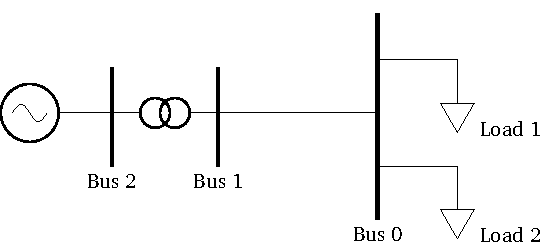
\includegraphics{tikz_graphics/images/sm_load_model.pdf}
    \vspace{12pt}
    \caption{Single line representation of a simple single machine load model; own illustration with characterstics from \quelle}
    \label{fig:single-line-voltage-stability}
\end{figure}

Further details about its configuration and simulation setup are included in \autoref{app:single-line-model}. It should be noted, that simple load models are not useful for simulation of this example network. Usually constant Z models are used as loads, therefore simulation results can be misleading and not showing desired effects or voltage instability mechanisms \quelle. \commenting{The simulation framework is extended with XX types of load models, to satisfy the requirements of the single machine load model, and a connected stability assessment.}

\subsubsection{IEEE Nine-Bus System}

\subsubsection{Nordic Test System}

%%%%%%%%%%%%%%%%%%%%%%%%%%%%%%%
%%%%%%%%%%%%%%%%%%%%%%%%%%%%%%%
\section{Validation Steps}

%%%%%%%%%%%%%%%%%%%%%%%%%%%%%%%
\subsection{Validation of the $\Pi$-Modeled Transformer with Variable Tap Position}

\begin{figure}[htb!]
    \centering
    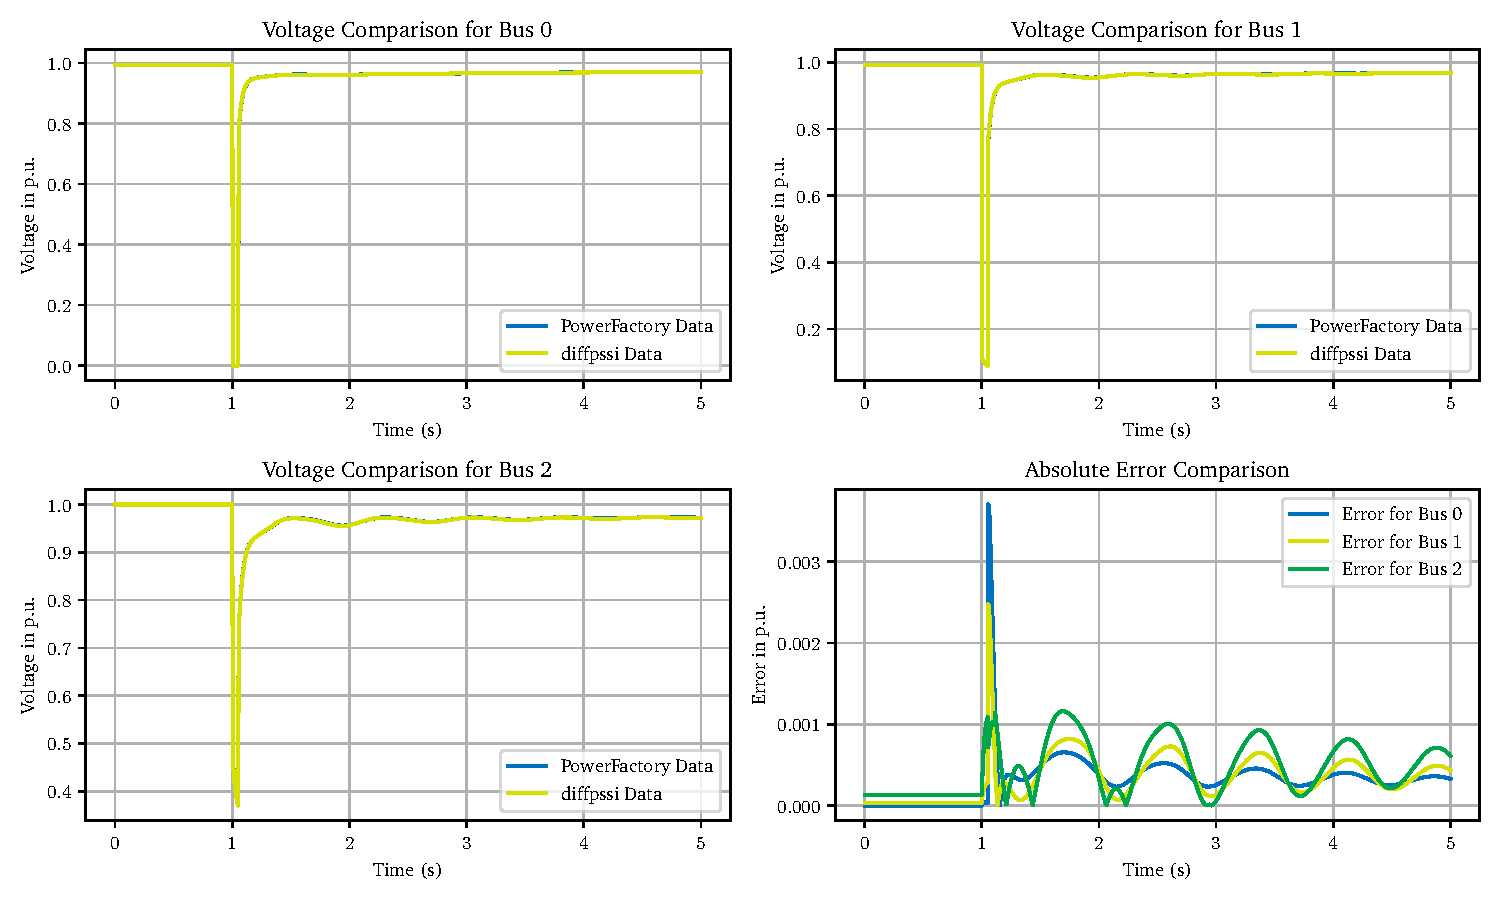
\includegraphics[width=\textwidth]{validation/comp_simple_pi.pdf}
    \caption{Comparison of the $\Pi$-modeled transformer in the \acs{SMIB} model between PowerFactory and the Python framework}
    \label{fig:comp-simple-pi}
\end{figure}

%%%%%%%%%%%%%%%%%%%%%%%%%%%%%%%
\subsection{Validation of the OLTC Control Schemes}

\subsubsection{Standard Discrete OLTC Control}

\subsubsection{Fast Switching OLTC Control}

%%%%%%%%%%%%%%%%%%%%%%%%%%%%%%%
\subsection{Voltage Stability Rating Plausibility}

\commenting{Place results here, looking at: off nominal tap ratio, and with off nominal phase shifting (e.g. $110^\circ$)}

%%%%%%%%%%%%%%%%%%%%%%%%%%%%%%%
\section{Discussion of Model Limitations and Improvements}

\section{Summary in Short and Simple Terms}